\chapter{Appendix}
\label{chap:appendix}
\section{Self Attention in the Decoder}
Whilst LayoutLMv2, BERT and most subsequent models do not have a decoder component as 
part of their architecture, for the sake of completeness and having described the encoder
from the transformers model, the decoder will be briefly described here.\\
The self attention mechanism in the decoder works in a very similar fashion to the encoder, but the inputs are different as per \Cref{fig:atn_decoder}.
\begin{figure}[H]
	\centering
	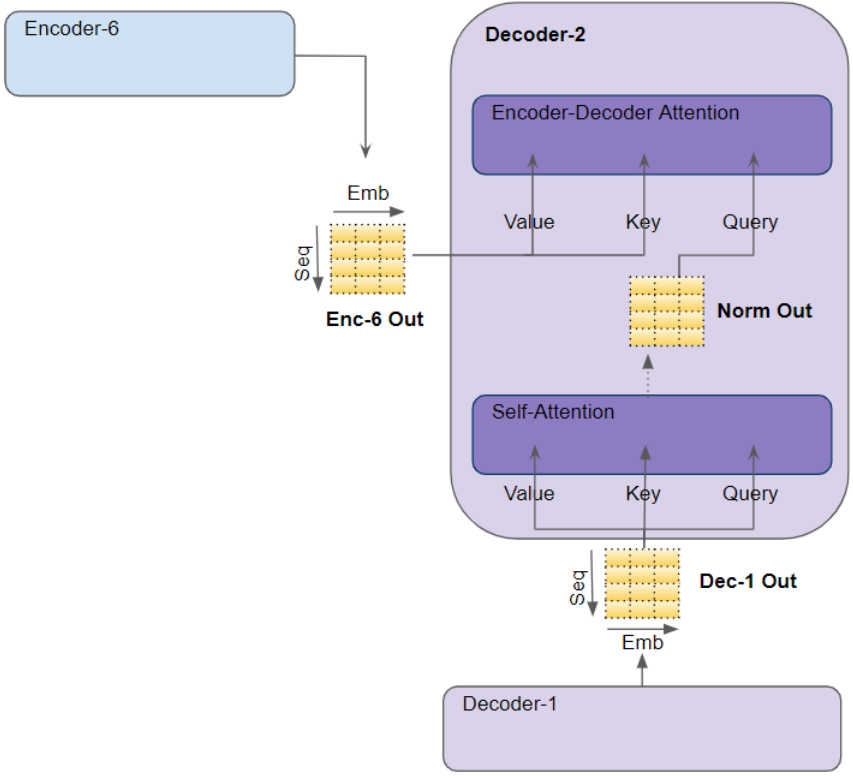
\includegraphics[width=0.8\textwidth]{figures/atn_decoder.png}
	\caption{Self Attention Mechanism for Decoder (source~\autocite{doshiTransformersExplainedVisually2021b}), depicting the resulting attention score.}
	\label{fig:atn_decoder}
\end{figure}
In the decoder the relevance of each word in the target sentence is computed with respect to every other word in the target sentence
as per \Cref{fig:decoder_self_atn}.
\begin{figure}[H]
	\centering
	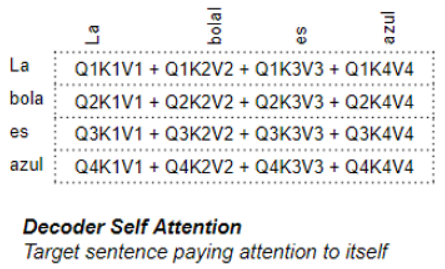
\includegraphics[width=0.6\textwidth]{figures/decoder_self_atn.png}
	\caption{Attention Mechanism for Encoder-Decoder in the decoder (source~\autocite{doshiTransformersExplainedVisually2021b}).}
	\label{fig:decoder_self_atn}
\end{figure}
\subsection{Attention in the Encoder-Decoder}
Again, very similar to the encoder attention but the Query is obtained from the target sentence and the Key and Value are obtained from the
source sentence. The goal is to compute the relevance of each word in the target sentence to each word in the source sentence.
\begin{figure}[H]
	\centering
	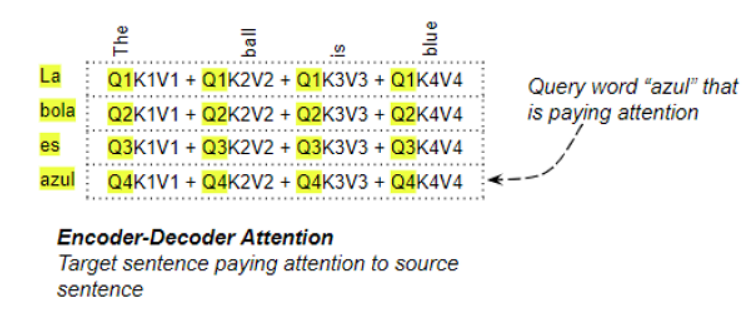
\includegraphics[width=0.9\textwidth]{figures/encoder_decoder_atn.png}
	\caption{Attention Mechanism for Encoder-Decoder (source~\autocite{doshiTransformersExplainedVisually2021b}). Same input
		and target as \Cref{fig:atn_decoder}.}
	\label{fig:atn_encoder_decoder}
\end{figure}